The objective is to determine the difference between the measured specific impulse and the theoretical values. To determine the experimental value for the specific impulse is a matter of measuring the force production of the nozzle and the change in mass of the system. This is done with the use of two force sensors. One measuring the change in mass of the $CO_2$ cylinder and the other measuring the force production of the nozzle. To determine the theoretical values for the same system requires measuring $T_c,\ T_e,\ P_c,\ and\ P_a$ where the ambient pressure is a constant and can be determined from the forecast that day. The same variables are needed for the predicted force equation. This information is coming from equations \ref{eq:RelevantNozzleForce} and \ref{eq:RelevantIsp}. It is important that these variables are represented well by the data collected, however the experimental setup used in the data collection presented here does a poor job of this. The setup and methods will be presented here along with solutions to the problems faced. 
\section{On-Ground Testing Rig}
A simplified schematic of the experimental apparatus is shown in figure \ref{fig:ApparatusSchem}.
\begin{figure}[h!]
\centering
\includegraphics[scale=.5]{Figures/Apparatus}
\caption{Simplified on-ground testing rig}
\label{fig:ApparatusSchem}
\end{figure}
\subsection{Hardware}
All of the parts, except the $CO_2$ adaptor and pressure transducer were ordered from McMaster-Carr. The adaptor was custom machined and the transducer was purchased from a third party seller with no datasheet provided. However, the voltage output from it varied linearly with pressure and could be calibrated with a simple linear regression function. The solenoid is a 24V DC 1000PSI solenoid valve, it was controlled by a simple digital signal run through a push pull (NPN-PNP pair) amplifier. Each temperature sensor was a type k thermocouple, interfacing with a XXXXXXX* breakout baord made by Adafruit. These breakoutboards interfaced with the data acquisition system via a 10-bit analog to digital converter. The force sensor used was a 1kg load cell interfacing with an HX711 (24-bit analog to digital converter) breakout board. The plumbing system used is 1/4" OD copper tubing with compression fittings that allowed adaptations between the copper pipe and the 1/8" National Pipe Threading (NPT) that was used for the non-pipe fittings. The choice of this plumbing system is the high pressure rating and relatively low weight. The most massive part of the system was the solenoid valve budgeting approximately 10\% ****CHECK THIS the maximum allowed weight of the HABP. On final thought, a choice was made to omit the flow controller because the mass flow rate should be limited by the nozzle throat.\footnote{This assumption will be discussed further in \ref{chap:Discussion}} For sake of simplicity these devices are referred to as "sensors" preceeded by the variable they measured. So $P_c$ sensor, $T_e$ sensor, $T_c$ sensor, and $F$ sensor. Additionally, $\gamma$ is dependent on temperature, but only changes slighty in the temperature differences noticed here. In later models, $\gamma$ will be set to be a function of temperature for greater accuracy. For now it is not necessary because the force has a small dependence on $\gamma$ compared to the temperature. A complete list of parts and schematics is available in section \ref{chap:Appendix}.
\subsubsection{Nozzle Manufacturing}
Several options were considered for the manufacturing of nozzles. These included the processes listed below:
\begin{itemize}
\item Fused deposition modeling (FDM) 3D printing
\item Resin 3D printing
\item Machining by hand
\item Modeling and casting by hand
\end{itemize}
However, in dealing with such small parts modeling and casting by hand was immediately discarded. Modeling differences of expansion ratios on the scale of parts of a millimeter was out of the question. Machining by hand is both costly in terms of money and time. Also, such small nozzles would present difficulties in the machining process. FDM 3D printing was by far the most accesible out of these, but there are problems related to both accuracy and actual function of the nozzles. FDM 3D printers typically use a .4mm nozzle. This limitation on accuracy is relatively large considering the nozzle throat is designed to by no larger than .625mm in diamter. Also, the .4mm nozzle refers to the actual size of the hole in the nozzle, \textit{not} the size of the filament extruded from the nozzle. FDM printers typically produce layer heights no smaller than .1mm. In addition to the problem of accuracy, the parts are relatively porous. The method of FDM printing calls for the extrusion of a hot filament onto a cooled layer of filament to produce a 3D model. This does well creating structural parts not dependent on high tolerances and do not need to be air-tight, but for a CGT nozzle it will not work well. Much of the fuel would be lost in the layers of the nozzle and the friction between the layers and exhaust gases would be moreso than any of the other methods. This leaves resin printing, often referred to as stereolithography (SLA) printing. This method has been out of reach for many in years past, but recent manufacturers have developed robust, inexpensive resin printers. These printers can provide layer heights of .01mm and do not rely on laying lines of hot filament on top of other layers. Rather, they use two main methods of creating the part. The cheaper versions use a 5.5x3.5in UV LCD screen with resolutions of approximately 2560x1400 pixels. These resolutions are much finer than the FDM printer's capabilities. Additionally, these layers are formed by a chemical curing of one layer of resin to the previous. Given no impurities in the resin, this will provide an air-tight seal in the part. Figure \ref{fig:PressurePrint} shows a pressure test that was performed on a printed part\footnote{This part has been soaked in IPA to reveal interior details of the part}, similar to the designed nozzles.
\begin{figure}[h!]
\centering
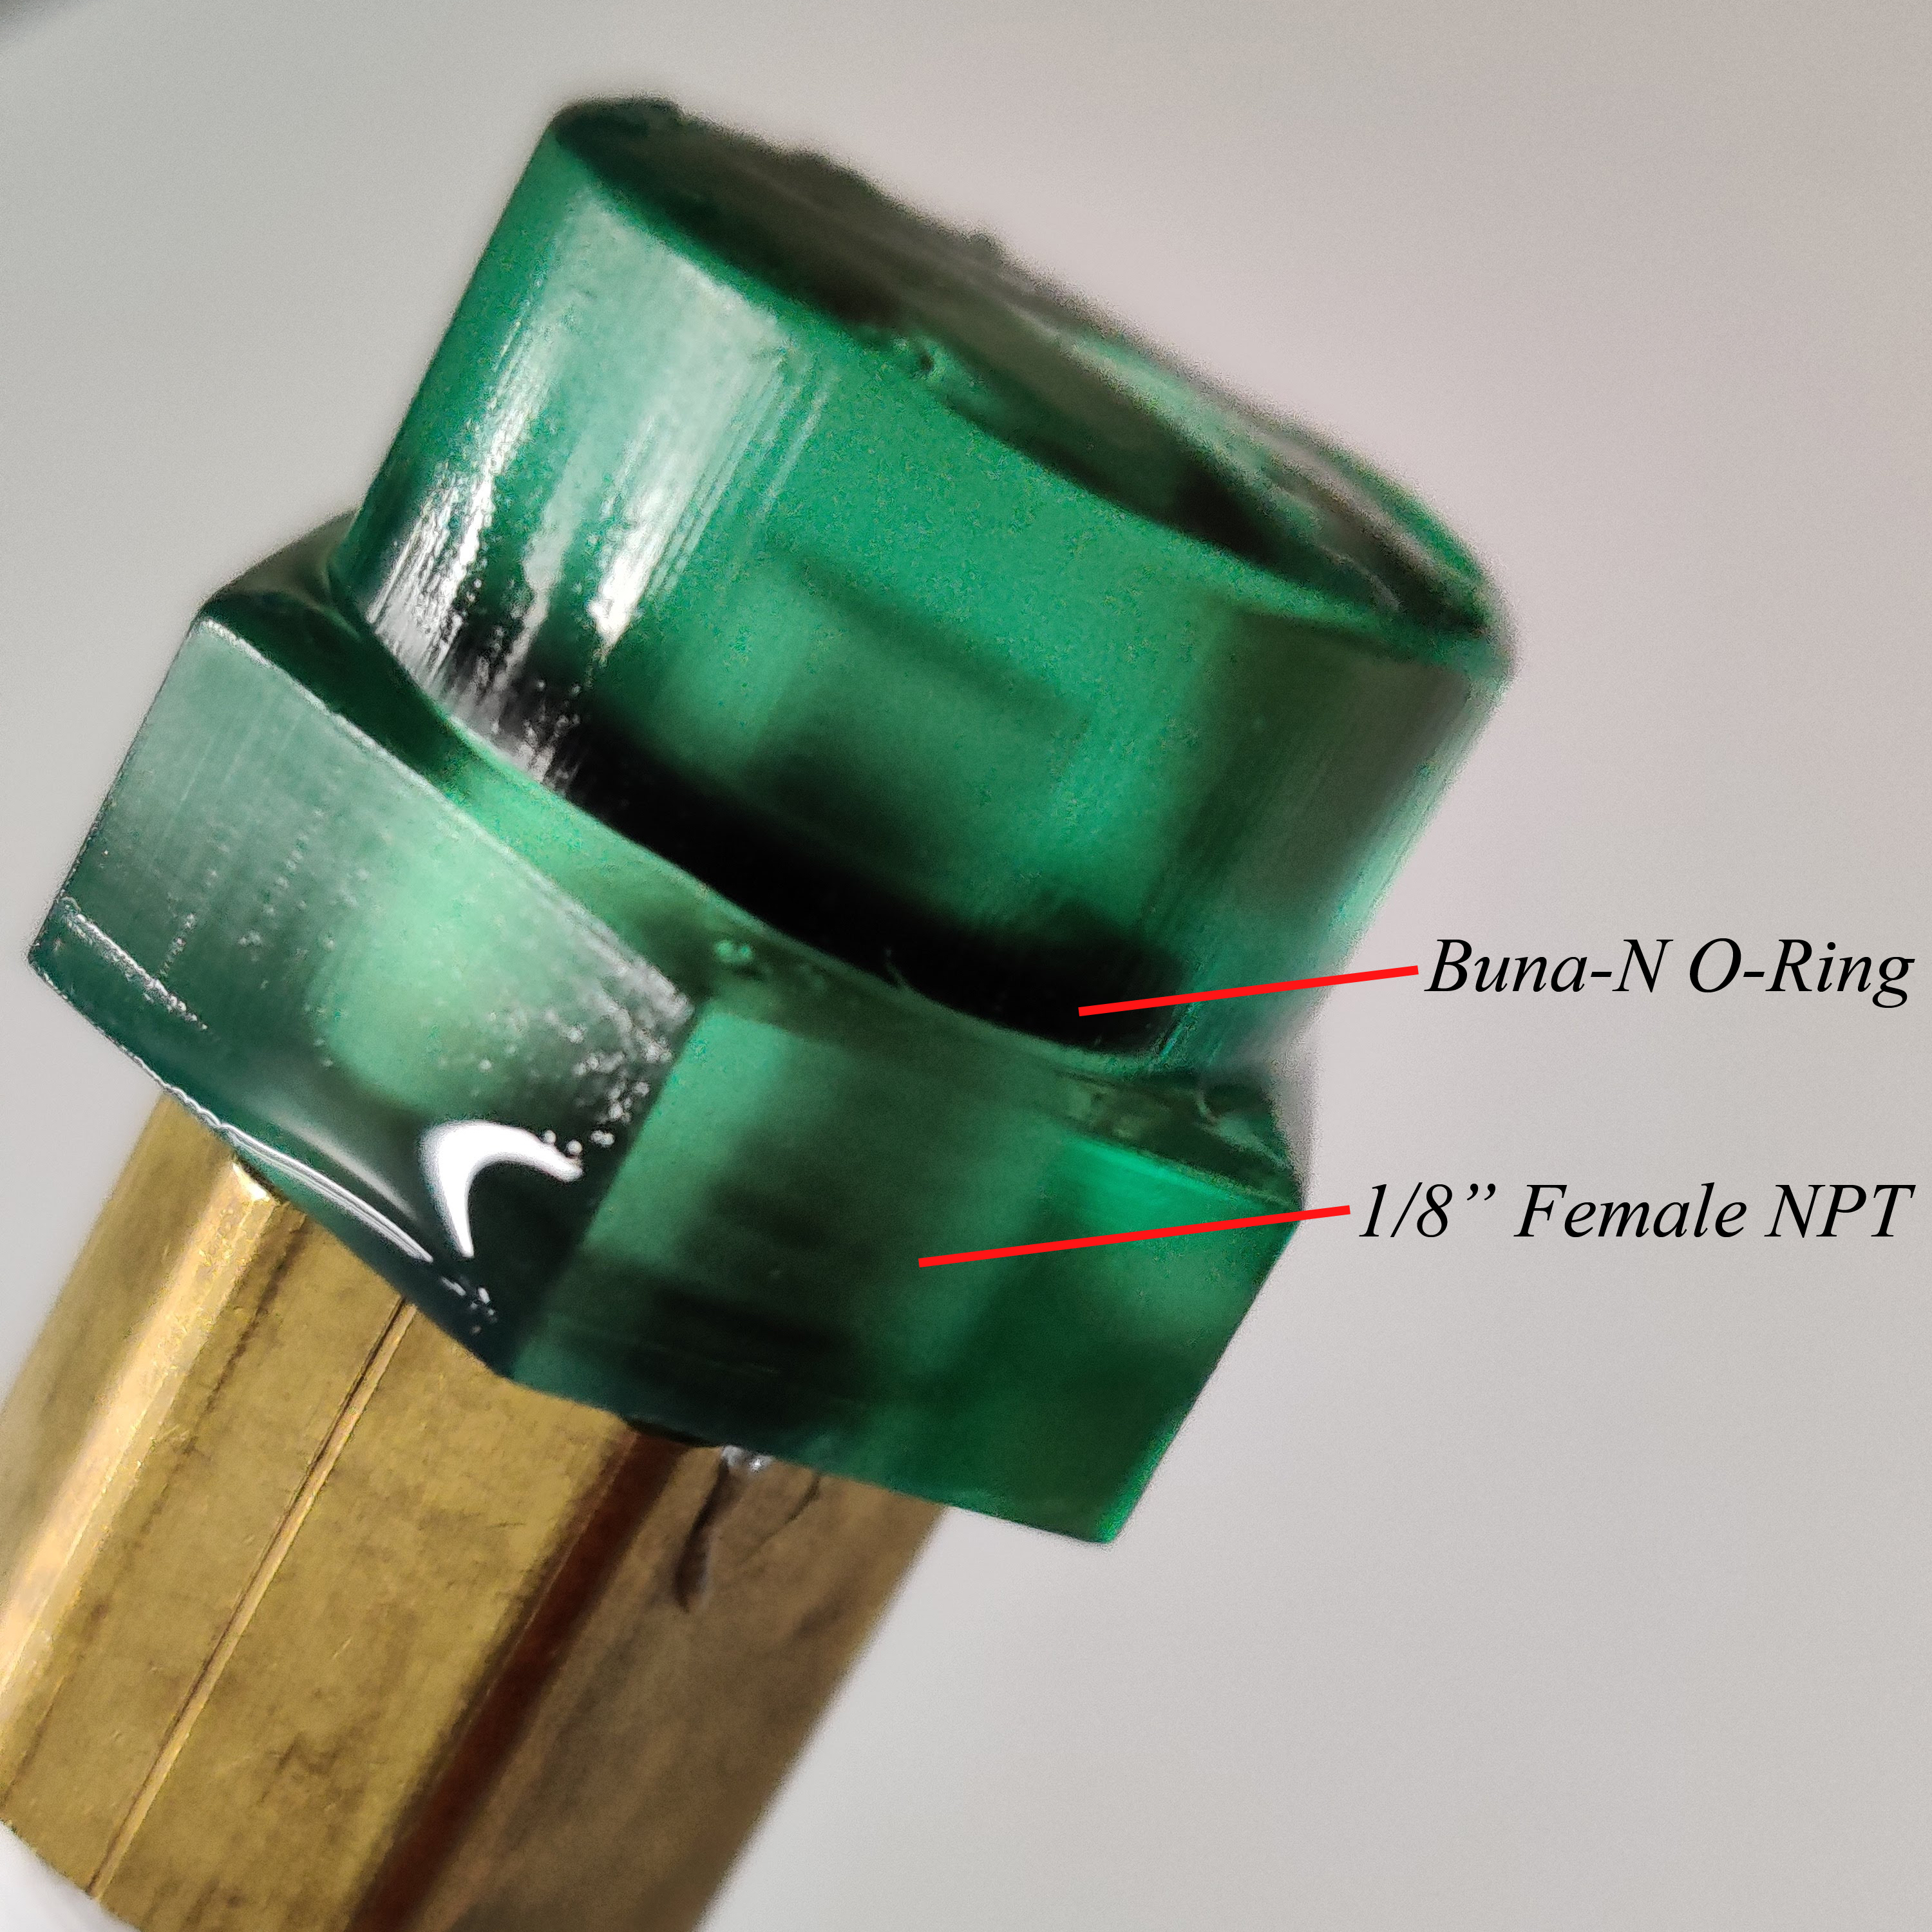
\includegraphics[width=10cm]{Figures/PressurePrint}
\caption{Pressure test of resin print from the ELEGOO MARS 3D printer}
\label{fig:PressurePrint}
\end{figure}
The part was essentially an end cap, filled in increments of 20psi up to 400psi. It was held at 400psi for 6 hours and it held that pressure with no noticeable change in the needle on the guage throughout that time. Similar tests with FDM printed parts held no pressure, even after being treated with an epoxy coating. For comparing the accuracy of the parts, several prints were done. Figure \ref{fig:Rooks} displays an example of the difference in detail and figure \ref{fig:RooksCompared} shows a closeup of the two at the same scale.\clearpage
\begin{figure}[h!]
\centering
\includegraphics[width=10cm]{Figures/RooksMarked}
\caption{Two 3D printed rooks for detail comparison. On left, resin and on right, FDM}
\label{fig:Rooks}
\end{figure}
\begin{figure*}[h!]
    \centering
    \begin{subfigure}[t]{0.5\textwidth}
        \centering
        \includegraphics[width=7cm]{Figures/RookClose}
        \caption{Resin printed rook closeup}
    \end{subfigure}%
    ~ 
    \begin{subfigure}[t]{0.5\textwidth}
        \centering
        \includegraphics[width=7cm]{Figures/FDMRookClose}
        \caption{FDM printed rook closeup}
    \end{subfigure}
    \caption{Rook closeups}
\label{fig:RooksCompared}
\end{figure*}
The layer height for the resin printed part was set to .05mm and the FDM is .25mm. The difference is easily noticed.\\
Nozzle design was done in two programs. First, the nozzle geometry was made in OpenSCAD. An open source program was used to set the parameters for the nozzle geometry. A .stl file was generated from OpenSCAD and imported into Blender. From here, the actual functional parts were added to the model like the hex flatends, NPT fitting, exterior walls, and labelling. Figure \ref{fig:BathingNozzles} shows several nozzles begin cleaned in isopropyl alcohol (IPA). The actual nozzle geometry can be seen while the part is covered in IPA.
\begin{figure}[h!]
\centering
\includegraphics[width=10cm]{Figures/BathingNozzles}
\caption{Several 3D printed nozzles bathing in IPA}
\label{fig:BathingNozzles}
\end{figure}
There were a total of 10 nozzle expansion ratios used with 2 trials each. The expansion ratio kept $A_t$ constant and varied $A_e$. There were 4 over expanded, 4 underexpanded, 1 optimum, and 1 with no expansion. The naming scheme goes something like ERT, where E stands for either U (Underexpanded), N (None), or O. O stands for either optimum or overexpanded. R is the ratio number (1-4) except in the case that there is no third character. In this case the O stands for optimum, which there is only one of. T stands for trial number which can be either 1 or 2. So for example, U22 is underexpanded, ratio number 2, trial number 2. O1 is optimum ratio, trial number 1. These are explicitly defined in the nomenclature section.%
\nomenclature{$O11$}{Overexpanded area ratio 1, trial 1}%
\nomenclature{$O12$}{Overexpanded area ratio 1, trial 2}%
\nomenclature{$O21$}{Overexpanded area ratio 2, trial 1}%
\nomenclature{$O22$}{Overexpanded area ratio 2, trial 2}%
\nomenclature{$O31$}{Overexpanded area ratio 3, trial 1}%
\nomenclature{$O32$}{Overexpanded area ratio 3, trial 2}%
\nomenclature{$O41$}{Overexpanded area ratio 4, trial 1}%
\nomenclature{$O42$}{Overexpanded area ratio 4, trial 2}%
\nomenclature{$U11$}{Underexpanded area ratio 1, trial 1}%
\nomenclature{$U12$}{Underexpanded area ratio 1, trial 2}%
\nomenclature{$U21$}{Underexpanded area ratio 2, trial 1}%
\nomenclature{$U22$}{Underexpanded area ratio 2, trial 2}%
\nomenclature{$U31$}{Underexpanded area ratio 3, trial 1}%
\nomenclature{$U32$}{Underexpanded area ratio 3, trial 2}%
\nomenclature{$U41$}{Underexpanded area ratio 4, trial 1}%
\nomenclature{$U42$}{Underexpanded area ratio 4, trial 2}%
\nomenclature{$O1$}{Optimum area ratio, trial 1}%
\nomenclature{$O2$}{Optimum area ratio, trial 2}%
\nomenclature{$N1$}{No expansion, trial 1}%
\nomenclature{$N2$}{No expansion, trial 2}
\subsubsection{Data Acquisition System}
The data acquisition system used here was a Raspberry Pi 3. The language used for scripting was Python. The project is hosted in a \href{https://github.com/maxmhuggins/RCS_HAB/tree/master/On_Ground_Testing/Code}{GitHub repository.} There are two main scripting sections in the repository. The scripting for the on-ground testing rig was developed first. In this section there are classes for each of the data sensors. These allow for simple implementation of each of them in the main experiment file. Essentially, each of these sensors is defined as an object in the experiment file and this is the file which initiates each trial. This is a relatively straightforward file that allows for the calibration of sensors if need be. Calibration for the $P_c$ sensor is a simple linear regression plotting observed voltages against the known pressures. The slope for this line allowed a conversion betwen observed ADC voltages and pressure values. The force sensor calibration used a method of known masses. Known masses are added to the scale and the voltage values were measured. These values are averaged and the unit conversion is formed by the division of the read voltage and the known mass. This is done for each mass and the unit conversions are averaged. The Adafruit breakout boards for the thermocouples do not require calibration.\\
The analysis for the data was done under another section and is all object oriented. These scripts include an analyzer class and a file for generating plots using the analyzer class. All of the computation is completed in the analyzer class and the figure generator is simply that, a figure generator.